% =========================================================================
% Auditing VLM Benchmarks for Free — NeurIPS 2026 Workshop submission (TAI-Eval, Sydney)
%
% BUILD: download the official NeurIPS 2026 style file (neurips_2026.sty) from
% the TAI-Eval CFP / neurips.cc and place it next to this file; check whether
% the workshop mandates its own style or page limit (typically 4-9 pages
% excluding references). Compile: pdflatex -> bibtex -> pdflatex x2.
%
% PLACEHOLDERS: every number still to be produced by the experiment runbook
% (docs/en/WorkPlan_TAI-Eval.md) is typeset as \ph{...}. Search for "\ph{"
% before submission — the paper must contain none.
% =========================================================================
\documentclass{article}

% Use the anonymous submission option unless the CFP says otherwise:
%   \usepackage{neurips_2026}          % camera-ready
%   \usepackage[preprint]{neurips_2026}
\usepackage[preprint]{neurips_2026}

\usepackage[utf8]{inputenc}
\usepackage[T1]{fontenc}
\usepackage{hyperref}
\usepackage{url}
\usepackage{booktabs}
\usepackage{amsfonts}
\usepackage{amsmath}
\usepackage{nicefrac}
\usepackage{microtype}
\usepackage{xcolor}
\usepackage{graphicx}
\usepackage{tikz}
\usetikzlibrary{positioning,arrows.meta,calc}
\usepackage{natbib}

% --- placeholder macro: red marker for numbers not yet produced ---
\newcommand{\ph}[1]{\textcolor{red}{\texttt{[#1]}}}

\title{Auditing VLM Benchmarks for Free:\\
Detecting Benchmark Pathologies from Existing Evaluation Runs}

% Anonymized for double-blind review; fill in for camera-ready.
\author{%
  Anonymous Authors\\
  Anonymous Affiliation\\
}

\begin{document}

\maketitle

\begin{abstract}
Leaderboards for vision--language models (VLMs) grow faster than the quality
of the underlying benchmarks is verified: mislabeled answers, questions
solvable without the image, and degenerate multiple-choice options remain
invisible in aggregate scores. We propose to treat the standard artifacts of
VLM evaluation---the per-question prediction files that toolkits already
save---as a free source of benchmark diagnostics. We integrate an audit layer
of six pathology detectors into VLMEvalKit \citep{vlmevalkit2024}: visual
dependency via matched full/blind runs, cross-model consensus against the
gold label, inter-model agreement (Fleiss'~$\kappa$), answer-position
distribution bias, near-duplicate distractors, and question--image relevance.
The layer runs as a single command over existing outputs and emits a
per-question audit report with severity levels. Auditing MMStar
\citep{mmstar2024} and HallusionBench \citep{hallusionbench2024} with
\ph{N=6} models, we find that \ph{XX.X}\% of MMStar questions are answered
identically by all models with and without the image---despite MMStar being
explicitly curated for vision-indispensability---and that on \ph{XX.X}\% of
questions a cross-model consensus contradicts the gold label
(\ph{NN} questions unanimously). Human verification of \ph{N=150} flagged
items puts detector precision at \ph{XX}\% (Cohen's $\kappa$=\ph{0.XX}
between annotators). Finally, we show that audit conclusions themselves are
sensitive to the answer-extraction/judge protocol: switching between exact
matching and an LLM judge changes the flagged set by \ph{XX}\%. We argue that
an audit report should accompany every leaderboard, and release code,
predictions, and reports.
\end{abstract}

\section{Introduction}
\label{sec:intro}

Progress claims about VLMs rest on benchmark accuracy, yet a growing body of
work documents that the benchmarks themselves are fragile: many items are
solvable without the image \citep{goyal2017vqa,mmstar2024,mmevalpro2024,datbench2026},
gold labels are frequently wrong \citep{northcutt2021pervasive,mmluredux2024,vendrow2025platinum},
multiple-choice formats carry position and selection biases
\citep{zheng2024selectors,mmbench2024,mmdetect2024}, and reported accuracies
are sensitive to prompt and extraction protocols \citep{rosenthal2025unexplored}.
Prior responses have been to build cleaner replacement benchmarks
\citep{mmstar2024,naturalbench2024,vendrow2025platinum,datbench2026} or
standalone flaw-flagging pipelines for text-only MCQ benchmarks
\citep{fantasticbugs2025,benchmarker2026}.

We take a complementary, infrastructure-first view. Every evaluation run of a
toolkit such as VLMEvalKit \citep{vlmevalkit2024} or LMMs-Eval
\citep{lmmseval2024} already persists per-question predictions, judged
correctness, and metadata. We show that this exhaust is sufficient to audit
the benchmark itself, at near-zero additional inference cost (only the blind
run adds inference, and it is text-only). Concretely, we contribute:

\begin{enumerate}
  \item \textbf{An audit layer inside VLMEvalKit} (\texttt{run.py --mode
  bench\_eval}): six detectors of benchmark pathologies operating purely as
  post-processing over saved prediction artifacts, with a documented
  \texttt{--blind} protocol that strips visual content uniformly for local
  and API models (Section~\ref{sec:method}).
  \item \textbf{A reflexive case study}: auditing MMStar---a benchmark
  constructed by filtering out text-solvable items---still surfaces
  \ph{XX.X}\% blind-solvable questions and \ph{XX.X}\% consensus--label
  conflicts; HallusionBench results in Section~\ref{sec:results}. We verify
  detector precision with two independent human annotators
  (Section~\ref{sec:validation}).
  \item \textbf{Judge sensitivity of audits}: the flagged sets shift by
  \ph{XX}\% between exact matching and LLM judges
  (Section~\ref{sec:judge}), extending protocol-sensitivity findings
  \citep{rosenthal2025unexplored} from accuracy to audit conclusions.
\end{enumerate}

We do not claim to discover these pathologies: blind-solvability and label
errors in VLM benchmarks were recently documented at scale by concurrent work
\citep{datbench2026}. Our claim is narrower and practical: these checks can
and should ship inside the evaluation infrastructure, so that every
evaluation run doubles as a benchmark audit.

\section{Related work}
\label{sec:related}

\paragraph{Benchmark pathologies.} Language priors in VQA were documented by
\citet{goyal2017vqa}; MMStar \citep{mmstar2024} and MMEvalPro
\citep{mmevalpro2024} showed that blind LLMs score non-trivially on
multimodal MCQ benchmarks; concurrent work measures visual dependence of
existing suites via blur ablations \citep{visualignorance2026} or
phrasing-controlled probes \citep{seeorguess2026}. Label errors destabilize
rankings \citep{northcutt2021pervasive}; re-annotation efforts include
MMLU-Redux \citep{mmluredux2024} and platinum benchmarks
\citep{vendrow2025platinum}. Position/selection bias in MCQ is established
for LLMs \citep{zheng2024selectors} and handled in MMBench via CircularEval
\citep{mmbench2024}; option-order sensitivity also signals contamination
\citep{mmdetect2024}.

\paragraph{Audit pipelines and toolkits.} Fantastic Bugs
\citep{fantasticbugs2025} mines response patterns to flag invalid questions
in nine text benchmarks; BenchMarker \citep{benchmarker2026} applies an
education-inspired rubric with LLM judges to text MCQ benchmarks; DatBench
\citep{datbench2026} audits 33 VLM datasets and releases a cleaned suite. Our
work differs on the deliverable: not a cleaned dataset nor a standalone
pipeline, but audit machinery embedded in a mainstream toolkit, reusable on
any benchmark/model set from artifacts the toolkit already saves. To our
knowledge no such layer exists for VLMEvalKit or LMMs-Eval
\citep{lmmseval2024}. Redundancy analyses over existing score matrices
\citep{redundancy2025} share the same reuse-the-exhaust spirit for a
different question.

\section{The audit layer}
\label{sec:method}

\begin{figure}[t]
  \centering
  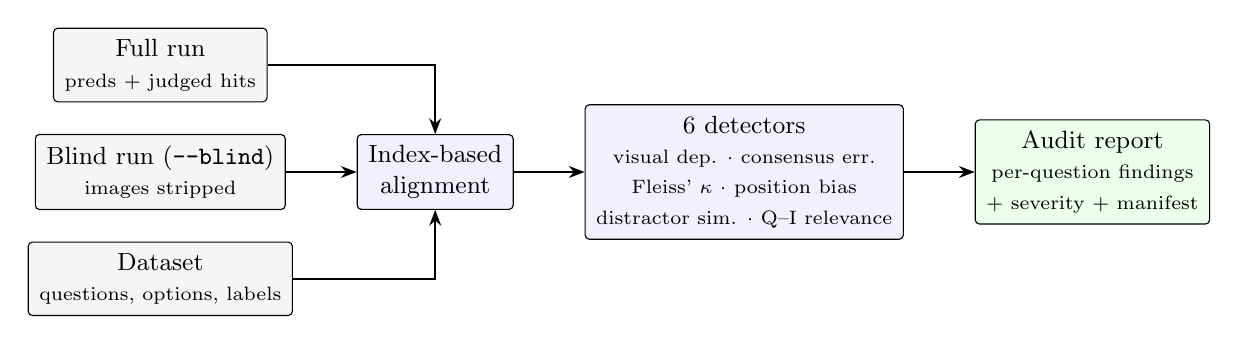
\begin{tikzpicture}[
      node distance=4mm and 7mm,
      box/.style={draw, rounded corners=1.5pt, align=center, font=\small, inner sep=4pt},
      lab/.style={font=\scriptsize\itshape},
      arr/.style={-{Stealth[length=2mm]}, thick}]
    \node[box, fill=black!4] (full) {Full run\\\scriptsize preds + judged hits};
    \node[box, fill=black!4, below=of full] (blind) {Blind run (\texttt{--blind})\\\scriptsize images stripped};
    \node[box, fill=black!4, below=of blind] (ds) {Dataset\\\scriptsize questions, options, labels};
    \node[box, right=9mm of blind, fill=blue!6] (align) {Index-based\\alignment};
    \node[box, right=9mm of align, fill=blue!6, minimum width=34mm] (det) {6 detectors\\\scriptsize visual dep. $\cdot$ consensus err.\\\scriptsize Fleiss' $\kappa$ $\cdot$ position bias\\\scriptsize distractor sim. $\cdot$ Q--I relevance};
    \node[box, right=9mm of det, fill=green!8] (rep) {Audit report\\\scriptsize per-question findings\\\scriptsize + severity + manifest};
    \draw[arr] (full.east) -| ($(align.north)+(0,2mm)$) -- (align.north);
    \draw[arr] (blind) -- (align);
    \draw[arr] (ds.east) -| ($(align.south)+(0,-2mm)$) -- (align.south);
    \draw[arr] (align) -- (det);
    \draw[arr] (det) -- (rep);
  \end{tikzpicture}
  \caption{The audit pipeline. Standard evaluation artifacts (full runs, plus
  one cheap text-only blind run) are aligned on dataset question ids and
  passed to six detectors; the output is a per-question audit report with
  severity levels and a reproducibility manifest (git commit, CLI arguments,
  generation parameters).}
  \label{fig:pipeline}
\end{figure}

\subsection{Inputs and the blind-run protocol}

The layer consumes the per-question result files of $n$ models
$\{f_m\}_{m=1}^{n}$ on one benchmark, each with raw \texttt{prediction},
gold \texttt{answer}, and (optionally) judged correctness \texttt{hit}. A
\emph{blind run} repeats inference with all visual content removed from every
prompt (text untouched), implemented centrally so that local and API models
are treated identically; blind artifacts receive a \texttt{\_blind} suffix
and live beside the full run. All frames are aligned on the dataset-level
question id---never on row order---and restricted to the shared id set.

\subsection{Detectors}
\label{sec:detectors}

Table~\ref{tab:detectors} summarizes the six detectors. Two design rules
matter for validity. (i)~\emph{Judge-free where possible}: consensus and
agreement detectors parse option letters from raw predictions (unparseable
predictions become an abstention sentinel excluded from votes), so they do
not inherit the judge; visual dependency and correctness agreement consume
judged labels and are analyzed for judge sensitivity in
Section~\ref{sec:judge}. (ii)~\emph{No ground-truth leakage}: model answers
are never back-filled from gold labels, regardless of judged correctness.

\begin{table}[t]
  \caption{Detector taxonomy. ``Judge-dep.'' marks detectors whose output
  depends on the answer-extraction/judge protocol.}
  \label{tab:detectors}
  \centering
  \small
  \begin{tabular}{lllc}
    \toprule
    Detector & Signal & Pathology flagged & Judge-dep. \\
    \midrule
    \texttt{visual\_dependency} & full vs.\ blind accuracy & text-solvable / image-harmful items & yes \\
    \texttt{consensus\_error} & majority vote vs.\ label & annotation-error candidates & no \\
    \texttt{fleiss\_kappa\_agreement} & inter-model $\kappa$ & unstable / ambiguous items & no \\
    \texttt{correctness\_agreement} & judged-correctness profile & difficulty / discrimination & yes \\
    \texttt{answer\_options\_distribution} & label-position histogram & position bias & no \\
    \texttt{distractor\_similarity} & pairwise option similarity & near-duplicate options & no \\
    \bottomrule
  \end{tabular}
\end{table}

For visual dependency, each question is categorized from model-averaged full
accuracy $a^F_q$ and blind accuracy $a^B_q$: \emph{visual-dependent}
($a^F_q{\ge}\theta_F$, $a^B_q{\le}\theta_B$), \emph{visual-supplement}
($a^F_q-a^B_q\ge\delta$), \emph{text-only} ($a^F_q\approx a^B_q$), and
\emph{conflicting} ($a^B_q>a^F_q+\delta$, i.e.\ the image hurts). Threshold
sensitivity is reported in Appendix~\ph{X}. Consensus errors are tiered:
\emph{very high} (all models agree on the same non-gold option), \emph{high}
(all models disagree with the gold label), \emph{medium} (qualified majority
disagrees).

\section{Experimental setup}
\label{sec:setup}

\textbf{Benchmarks.} MMStar (1{,}500 MCQ items; curated for
vision-indispensability) and HallusionBench (951 yes/no items; designed
around visual illusions and language priors). \textbf{Models.} \ph{list the
final pool: e.g.\ InternVL3-8B, Ristretto-3B, Qwen2.5-VL-7B-Instruct,
LLaVA-OneVision-7B, GPT-5-nano, GPT-4.1-mini} ($n=\ph{6}$), spanning
\ph{2--8}B open models and API models. \textbf{Decoding.} Greedy
(\texttt{do\_sample=False}, temperature $0$) for all main runs; run-to-run
variance under default sampling is quantified for one model in
Appendix~\ph{X} (\ph{3} repeats). \textbf{Judges.} Exact matching and
\texttt{gpt-4o-mini} (primary), plus \ph{second LLM judge} for the
sensitivity study; identical judge for full and blind variants.
\textbf{Reproducibility.} Every run records git commit, CLI arguments, and
generation parameters in its manifest; audits are deterministic given the
artifacts. Total compute: \ph{XX} A100-hours + \ph{\$XX} API spend.

\section{Results}
\label{sec:results}

\begin{table}[t]
  \caption{Main audit results (\ph{fill from
  \texttt{reports/*/}}). VD = visual-dependent, TO = text-only, CF =
  conflicting visual signal; CE = consensus-error rate (unanimous in
  parentheses).}
  \label{tab:main}
  \centering
  \small
  \begin{tabular}{lcccccc}
    \toprule
    Benchmark & VD (\%) & Suppl.\ (\%) & TO (\%) & CF (\%) & CE (\%) & Fleiss' $\kappa$ \\
    \midrule
    MMStar         & \ph{XX.X} & \ph{XX.X} & \ph{XX.X} & \ph{X.X} & \ph{XX.X} (\ph{X.X}) & \ph{0.XX} \\
    HallusionBench & \ph{XX.X} & \ph{XX.X} & \ph{XX.X} & \ph{X.X} & \ph{XX.X} (\ph{X.X}) & \ph{0.XX} \\
    \bottomrule
  \end{tabular}
\end{table}

\textbf{Even curated benchmarks retain text-solvable items.}
\ph{One paragraph: the headline MMStar text-only rate with a 95\% bootstrap
CI over questions, leave-one-model-out range, and 2--3 concrete example
questions (with ids) in Appendix. Compare against the MMStar authors' own
curation procedure: overlap of our text-only set with their reported
leakage analysis.}

\textbf{Label-error candidates.} \ph{One paragraph: consensus-error rates,
the unanimous subset, and what human verification showed (link to
Section~\ref{sec:validation}); 2--3 worked examples of confirmed annotation
errors with question ids.}

\textbf{The image can hurt.} \ph{One paragraph on the conflicting category
(blind $>$ full): rate, examples, hypothesis (misleading figures,
illusion-style items in HallusionBench).}

\begin{figure}[t]
  \centering
  % Generated by scripts/audit_paper_assets.py -> figures/fig_scatter_mmstar.pdf
  \fbox{\parbox[c][4.2cm][c]{0.92\linewidth}{\centering \ph{Figure: per-question
  scatter of full vs.\ blind accuracy on MMStar (x = blind, y = full, jittered,
  colored by category, marginal histograms). One panel per benchmark.}}}
  \caption{Full vs.\ blind per-question accuracy (\ph{n} models). Points on
  the diagonal need no image; points below it are \emph{harmed} by the image.}
  \label{fig:scatter}
\end{figure}

\subsection{Human verification of flagged items}
\label{sec:validation}

Two annotators independently reviewed \ph{150} flagged items (\ph{50}
unanimous/high consensus errors, \ph{50} visual-dependent/text-only
disputes, \ph{50} near-duplicate distractors) under the protocol in
Appendix~\ph{X}. Precision: consensus errors \ph{XX}\%, text-only \ph{XX}\%,
distractors \ph{XX}\%; inter-annotator agreement Cohen's
$\kappa=\ph{0.XX}$. \ph{One paragraph: main false-positive modes (e.g.\
judge extraction failures masquerading as consensus errors) and what they
imply for using the audit reports.}

\begin{figure}[t]
  \centering
  % Generated by scripts/audit_paper_assets.py -> figures/fig_precision.pdf
  \fbox{\parbox[c][3.4cm][c]{0.92\linewidth}{\centering \ph{Figure: bar chart of
  detector precision from human verification, with Wilson 95\% intervals; one
  group per detector, annotator-1 vs annotator-2 vs adjudicated.}}}
  \caption{Detector precision under human verification.}
  \label{fig:precision}
\end{figure}

\subsection{Audit conclusions are judge-dependent}
\label{sec:judge}

We recompute all judge-dependent statistics under \ph{3} protocols (exact
matching, \texttt{gpt-4o-mini}, \ph{judge 3}) on identical predictions.
\ph{One paragraph + small table: Jaccard overlap of flagged sets across
judges per detector; which categories are stable (unanimous consensus
errors: \ph{XX}\% stable) and which flip (text-only vs supplement boundary:
\ph{XX}\% stable). Note that blind-run predictions are judged
disproportionately differently: \ph{evidence}.} This extends
protocol-sensitivity results \citep{rosenthal2025unexplored} from accuracy
numbers to audit outcomes: benchmark-quality claims must state their judge.

\section{Limitations}
\label{sec:limitations}

(i)~Detector thresholds are heuristics; we report sensitivity but do not
calibrate them against a gold standard beyond our \ph{150}-item verification.
(ii)~With $n$ models, per-question accuracies live on an $(n{+}1)$-point
grid; categories are noisy for small $n$ and we report leave-one-model-out
stability rather than formal significance. (iii)~High blind accuracy mixes
language priors with training-data contamination; our protocol cannot
separate them (cf.\ \citealp{mmdetect2024}). (iv)~Judge-dependent detectors
inherit judge errors; we measure but do not eliminate this. (v)~The layer
currently targets MCQ/yes-no benchmarks; free-form generation benchmarks
need different detectors. (vi)~Case studies cover two benchmarks; claims are
about the audit machinery, not about all VLM benchmarks.

\section{Conclusion}

Benchmark audits need not be a separate research project: the artifacts that
evaluation toolkits already save, plus one cheap text-only run, suffice to
flag text-solvable items, annotation-error candidates, and degenerate
options---with measured precision and stated judge sensitivity. We release
the audit layer inside VLMEvalKit, all predictions, and per-question reports,
and argue that leaderboards should ship with audit reports attached.

\begin{ack}
\ph{Funding / compute acknowledgements — omit in anonymized submission.}
\end{ack}

\bibliographystyle{plainnat}
\bibliography{references}

\appendix

\section{Annotation protocol}
\ph{Copy the protocol from docs/en/AnnotationProtocol.md: item sampling,
instructions, decision categories, adjudication rule, time spent.}

\section{Threshold sensitivity}
\ph{Heatmap/table: category shares as functions of
$(\theta_F,\theta_B,\delta)$ over a grid.}

\section{Run-to-run variance}
\ph{Table: 3 sampled repeats of one model; per-question flip rate; effect on
audit categories.}

\section{Worked examples}
\ph{6--10 flagged questions with images, options, model votes, gold label,
and human verdicts (respect dataset licenses when reproducing images).}

\section{NeurIPS paper checklist}
\ph{Fill the official checklist: claims match evidence; limitations section
included; no human-subjects concerns beyond two-author annotation; licenses
of MMStar/HallusionBench respected; code and artifacts released.}

\end{document}
